\documentclass[a4paper]{article}
%\VignetteIndexEntry{gridBase}
\newcommand{\grid}{{\tt grid}}
\newcommand{\gridBase}{{\tt gridBase}}
\newcommand{\lattice}{{\tt lattice}}
\newcommand{\R}{{\tt R}}
\setlength{\parindent}{0in}
\setlength{\parskip}{.1in}

\newcommand{\aside}[1]{\begin{list}{}
                                   {\setlength{\leftmargin}{1in}
                                    \setlength{\rightmargin}{1in}
                                    \setlength{\itemindent}{0in}}
                       \item {\sc Aside:} {\it #1}
                       \end{list}}

\title{Integrating Grid Graphics Output \\ with Base Graphics Output}
\author{Paul Murrell}

\usepackage{/home/rdev/paul/Research/Rstuff/r-devel-grid/R/share/texmf/Sweave}
\begin{document}
\maketitle

The \grid{} graphics package\cite{Rnews:Murrell:2002}
 is much more powerful than the standard \R{} graphics system
(hereafter ``base 
graphics'') when it comes to combining and arranging graphical elements.
It is possible to create a greater variety of graphs more easily with 
\grid{} (see, for example, Deepayan Sarkar's \lattice{} 
package\cite{Rnews:Sarkar:2002}).
However,  there are very many plots based on base graphics (e.g., 
biplots), that have not been implemented in \grid{}, and the
task of reimplementing these in \grid{} is extremely daunting.
It would be nice to be able to combine the 
ready-made base plots with the sophisticated arrangement features
of grid.

This document describes the \gridBase{} package which provides
 some support for combining grid and base
graphics output.

\section*{Annotating base graphics using \grid{}}

The \gridBase{} package has one function, \verb|baseViewports()|, 
that supports 
adding \grid{} output to a base graphics plot.
This function creates a set of \grid{} 
viewports that correspond to the current
base plot.
This allows simple annotations such as adding lines and text using \grid{}'s
units to locate them relative to 
a wide variety of coordinate systems, or something
more complex involving
pushing further \grid{} viewports.

{\tt baseViewports()} returns a list of three grid viewports.  The first 
corresponds to the base ``inner'' region.  This viewport is relative to
 the entire device; it only makes sense to push this viewport
from the ``top level'' (i.e., only when no other viewports have been 
pushed).
The second viewport corresponds to the base ``figure'' region
and is relative to the inner region;  it only makes sense to push it
after the ``inner'' viewport has been pushed.  The third 
viewport corresponds to the 
base ``plot'' region  and is relative to the figure region;  it only
makes sense to push it after the other two viewports have been pushed in the
correct order.  

A simple application of this facility involves adding text to 
the margins of a base plot at an arbitrary orientation.  The base
function \verb|mtext()| allows text to be located  in terms of a number
of lines away from the plot region, but only at rotations of 0 or
90 degrees.  The base \verb|text()| function allows arbitrary rotations,
but only locates text relative to the user coordinate system in effect
in the plot region (which is inconvenient for locating text in the
margins of the plot).  By contrast, the \grid{} function 
\verb|grid.text()| allows arbitrary rotations and can be used in 
any \grid{} viewport.  In the following code we first create a base plot,
leaving off the tick labels. 

\begin{Schunk}
\begin{Sinput}
> midpts <- barplot(1:10, axes = FALSE)
> axis(2)
> axis(1, at = midpts, labels = FALSE)
\end{Sinput}
\end{Schunk}
Next we  use \verb|baseViewports()| to 
create grid viewports that correspond to the base plot and we push
those viewports\footnote{The {\tt par(new=TRUE)}
is necessary currently because the first grid action will
try to move to a new page;  it should be possible to remove
this step in future versions of \R{}.}.

\begin{Schunk}
\begin{Sinput}
> vps <- baseViewports()
> par(new = TRUE)
> pushViewport(vps$inner, vps$figure, vps$plot)
\end{Sinput}
\end{Schunk}
Finally, we draw rotated labels using 
\verb|grid.text()| (and pop the viewports to clean up after ourselves).

\begin{Schunk}
\begin{Sinput}
> grid.text(c("one", "two", "three", "four", "five", "six", "seven", 
+     "eight", "nine", "ten"), x = unit(midpts, "native"), y = unit(-1, 
+     "lines"), just = "right", rot = 60)
> popViewport(3)
\end{Sinput}
\end{Schunk}
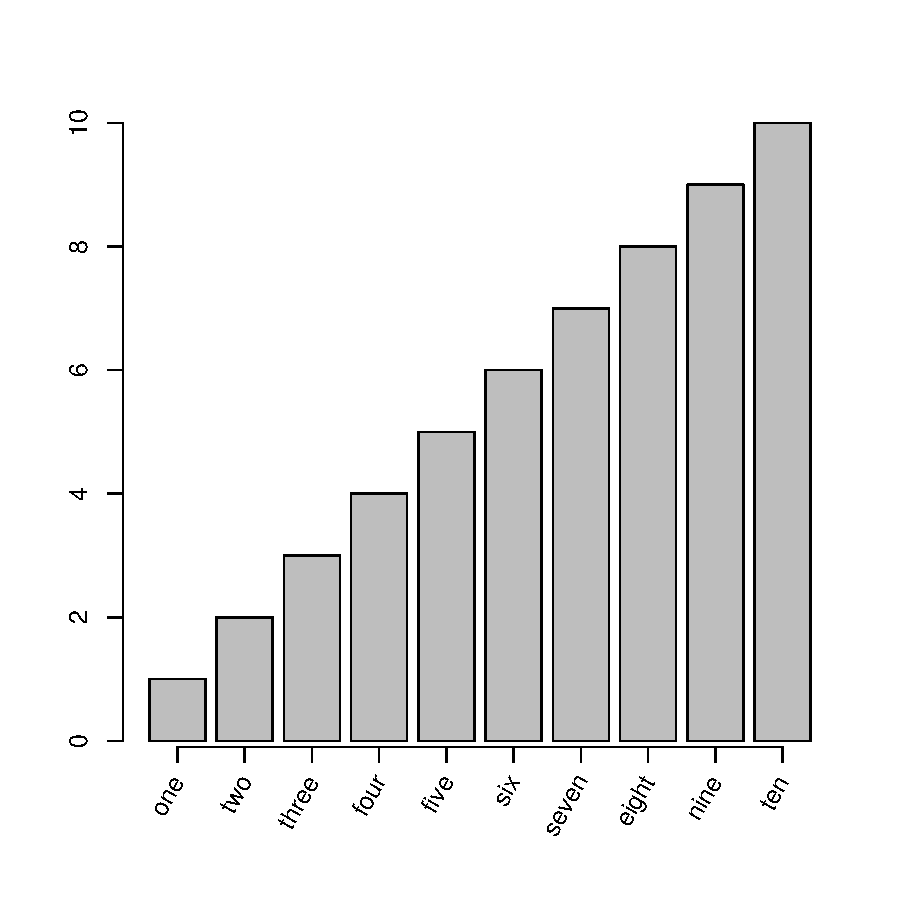
\includegraphics{gridBase-005}

The next example is a bit more complicated because it involves 
embedding \grid{} viewports within a base graphics plot.
The dataset is a snapshot of wind speed, wind direction, and temperature
at several weather stations in the South China Sea, south west of 
Japan\footnote{Obtained from the CODIAC web site:
{\tt http://www.joss.ucar.edu/codiac/codiac-www.html}.  The file
{\tt chinasea.txt} is in the {\tt gridBase/doc} directory.}.
\grid{} is used to produce novel plotting symbols for a standard
base plot.

First of all, we need to define the novel plotting symbol.  This consists
of a dot at the data location, with a thermometer extending ``below''
and an arrow extending ``above''.  The thermometer is used to encode 
temperature 
and the arrow is used to indicate wind speed 
(both scaled to [0, 1]).

\begin{Schunk}
\begin{Sinput}
> novelsym <- function(speed, temp, width = unit(3, "mm"), length = unit(0.5, 
+     "inches")) {
+     grid.rect(height = length, y = 0.5, just = "top", width = width, 
+         gp = gpar(fill = "white"))
+     grid.rect(height = temp * length, y = unit(0.5, "npc") - 
+         length, width = width, just = "bottom", gp = gpar(fill = "grey"))
+     grid.arrows(x = 0.5, y = unit.c(unit(0.5, "npc"), unit(0.5, 
+         "npc") + speed * length), length = unit(3, "mm"), type = "closed", 
+         gp = gpar(fill = "black"))
+     grid.points(unit(0.5, "npc"), unit(0.5, "npc"), size = unit(2, 
+         "mm"), pch = 16)
+ }
\end{Sinput}
\end{Schunk}
Now we read in the data and generate a base plot, but plot no points.

\begin{Schunk}
\begin{Sinput}
> chinasea <- read.table("chinasea.txt", header = TRUE)
> plot(chinasea$lat, chinasea$long, type = "n", xlab = "latitude", 
+     ylab = "longitude", main = "China Sea Wind Speed/Direction and Temperature")
\end{Sinput}
\end{Schunk}
Now we use \verb|baseViewports()| to align a \grid{} viewport
with the plot region, and draw the symbols by creating a 
\grid{} viewport per $(x, y)$ location (we rotate the viewport to
represent the wind direction).

\begin{Schunk}
\begin{Sinput}
> speed <- 0.8 * chinasea$speed/14 + 0.2
> temp <- chinasea$temp/40
> vps <- baseViewports()
> par(new = TRUE)
> pushViewport(vps$inner, vps$figure, vps$plot)
> for (i in 1:25) {
+     pushViewport(viewport(x = unit(chinasea$lat[i], "native"), 
+         y = unit(chinasea$long[i], "native"), angle = chinasea$dir[i]))
+     novelsym(speed[i], temp[i])
+     popViewport()
+ }
> popViewport(3)
\end{Sinput}
\end{Schunk}
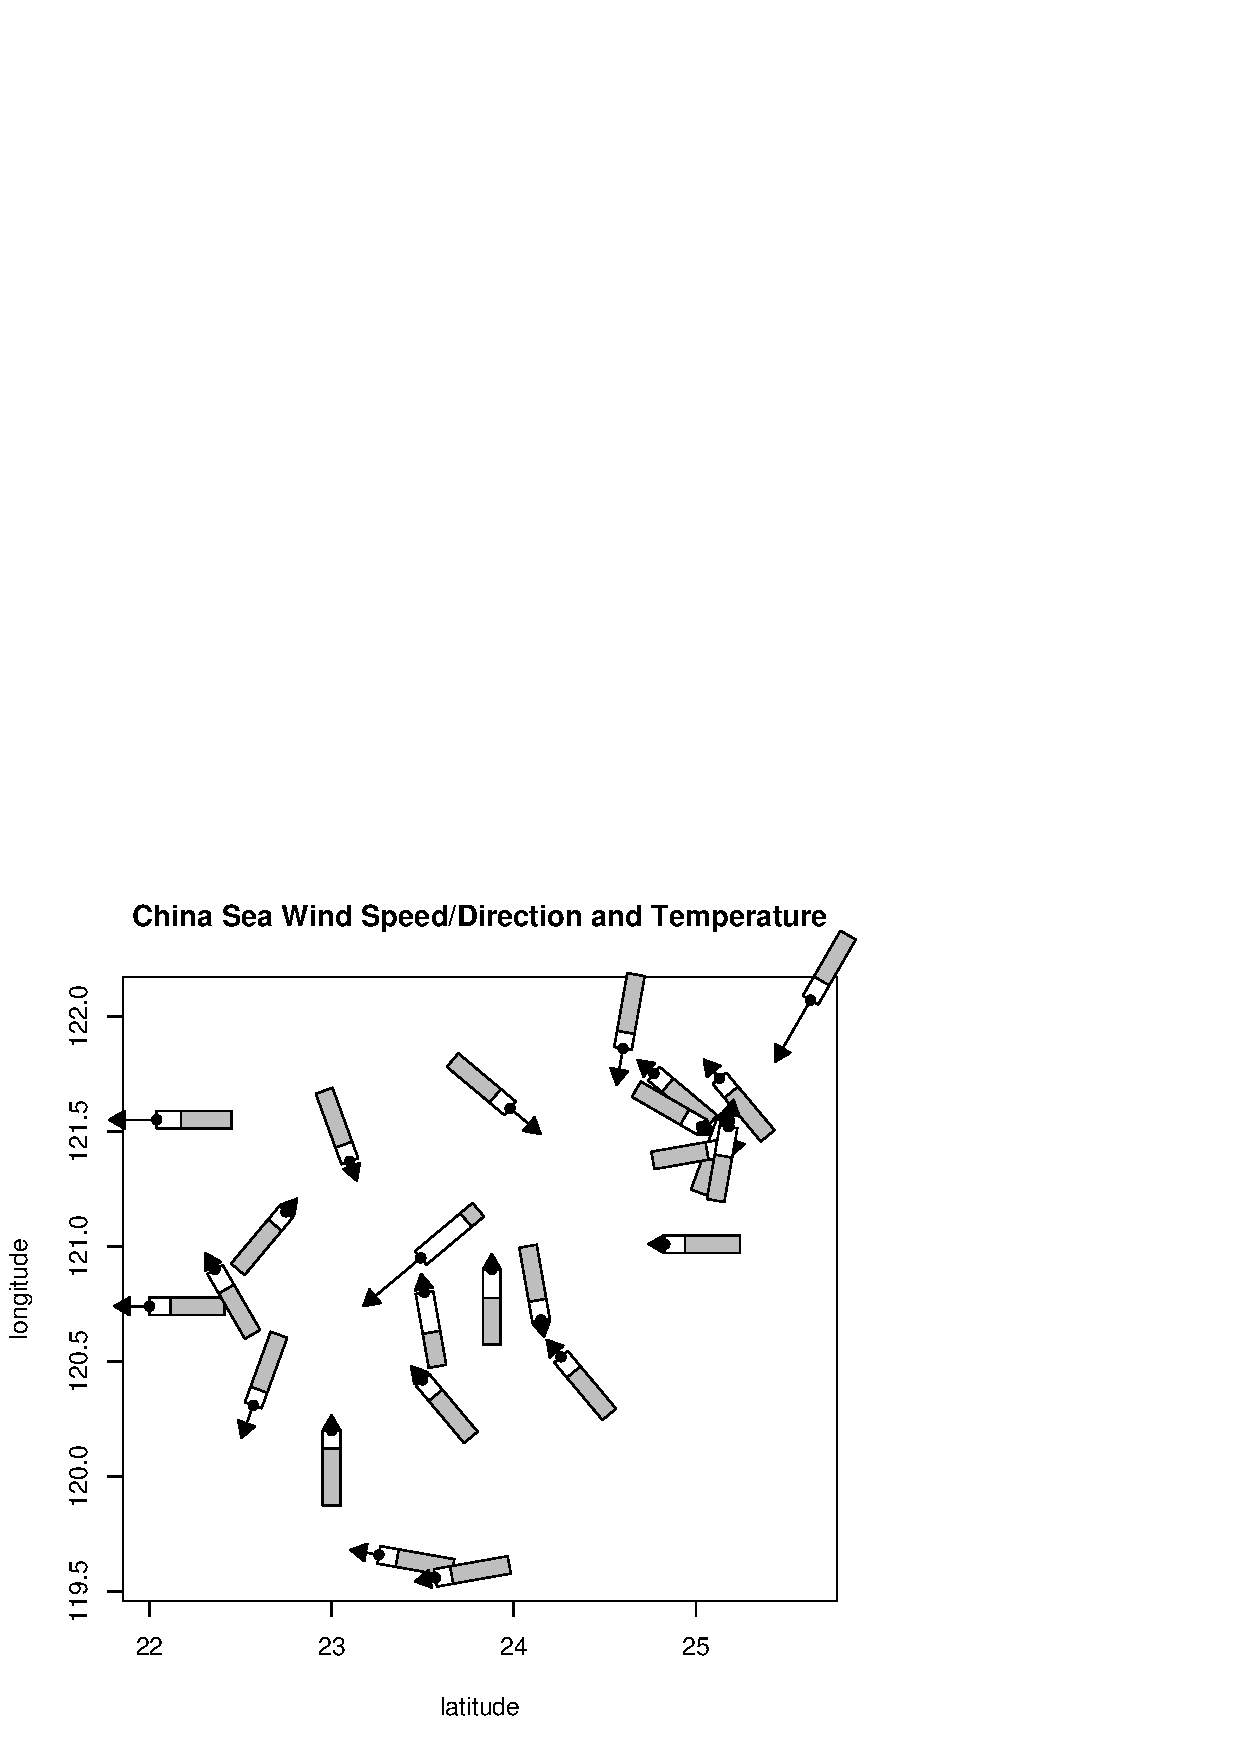
\includegraphics{gridBase-009}
\section*{Embedding base graphics plots in \grid{} viewports}

\gridBase{} provides several functions for adding base graphics 
output to \grid{} output.  There are three functions that allow
base plotting regions to be aligned with the current \grid{} 
viewport;  this makes it possible to draw one or more base graphics plots 
within
a \grid{} viewport.  The fourth function provides a set of
graphical parameter settings so that base {\tt par()} settings
can be made to correspond to some of\footnote{Only {\tt lwd},
{\tt lty}, {\tt col} are available yet.  More should be available in
future versions.} the current \grid{} graphical parameter settings.

The first three functions are \verb|gridOMI()|, \verb|gridFIG()|,
and \verb|gridPLT()|.  They return the appropriate
\verb|par()| values for setting the base ``inner'', ``figure'',
and ``plot'' regions, respectively.

The main usefulness of these functions is to allow you to create a
complex layout using \grid{} and then draw a base plot within 
relevant elements of that layout.  The following example
uses this idea to create a \lattice{} plot where the panels contain 
dendrograms drawn using base graphics functions\footnote{Recall
that \lattice{} is built on \grid{} so the panel region in
a \lattice{} plot is a \grid{} viewport.}.

First of all, we create a dendrogram and cut it into four 
subtrees\footnote{the data and cluster analysis are copied from the example
in {\tt help(plot.dendrogram)}.}.

\begin{Schunk}
\begin{Sinput}
> data(USArrests)
> hc <- hclust(dist(USArrests), "ave")
> dend1 <- as.dendrogram(hc)
> dend2 <- cut(dend1, h = 70)
\end{Sinput}
\end{Schunk}
Now we create some dummy variables which correspond to the four subtrees.

\begin{Schunk}
\begin{Sinput}
> x <- 1:4
> y <- 1:4
> height <- factor(round(unlist(lapply(dend2$lower, attr, "height"))))
\end{Sinput}
\end{Schunk}
Next we define a \lattice{} panel function to draw the dendrograms.
The first thing this panel function does is push a viewport
that is smaller than the viewport \lattice{} creates for the panel;
the purpose is to ensure there is enough room for the labels on
the dendrogram.  The \verb|space| variable contains a measure
of the length of the longest label.
The panel function then calls \verb|gridPLT()|
and makes the base plot region correspond to the 
viewport we have just pushed.  Finally, we
call the base \verb|plot()| function to draw the 
dendrogram (and pop the viewport we pushed)\footnote{The {\tt grid.rect()}
call is just to show the extent of the extra viewport we pushed.}.

\begin{Schunk}
\begin{Sinput}
> space <- max(unit(rep(1, 50), "strwidth", as.list(rownames(USArrests))))
> dendpanel <- function(x, y, subscripts, ...) {
+     pushViewport(viewport(y = space, width = 0.9, height = unit(0.9, 
+         "npc") - space, just = "bottom"))
+     grid.rect(gp = gpar(col = "grey", lwd = 5))
+     par(plt = gridPLT(), new = TRUE, ps = 10)
+     plot(dend2$lower[[subscripts]], axes = FALSE)
+     popViewport()
+ }
\end{Sinput}
\end{Schunk}
Finally, we draw a \lattice{} xyplot, using \lattice{} to set up the
arrangement of panels and strips and our panel function to draw
a base dendrogram in each panel.

\begin{Schunk}
\begin{Sinput}
> library(lattice)
> xyplot(y ~ x | height, subscripts = TRUE, xlab = "", ylab = "", 
+     strip = function(...) {
+         strip.default(style = 4, ...)
+     }, scales = list(draw = FALSE), panel = dendpanel)
\end{Sinput}
\end{Schunk}
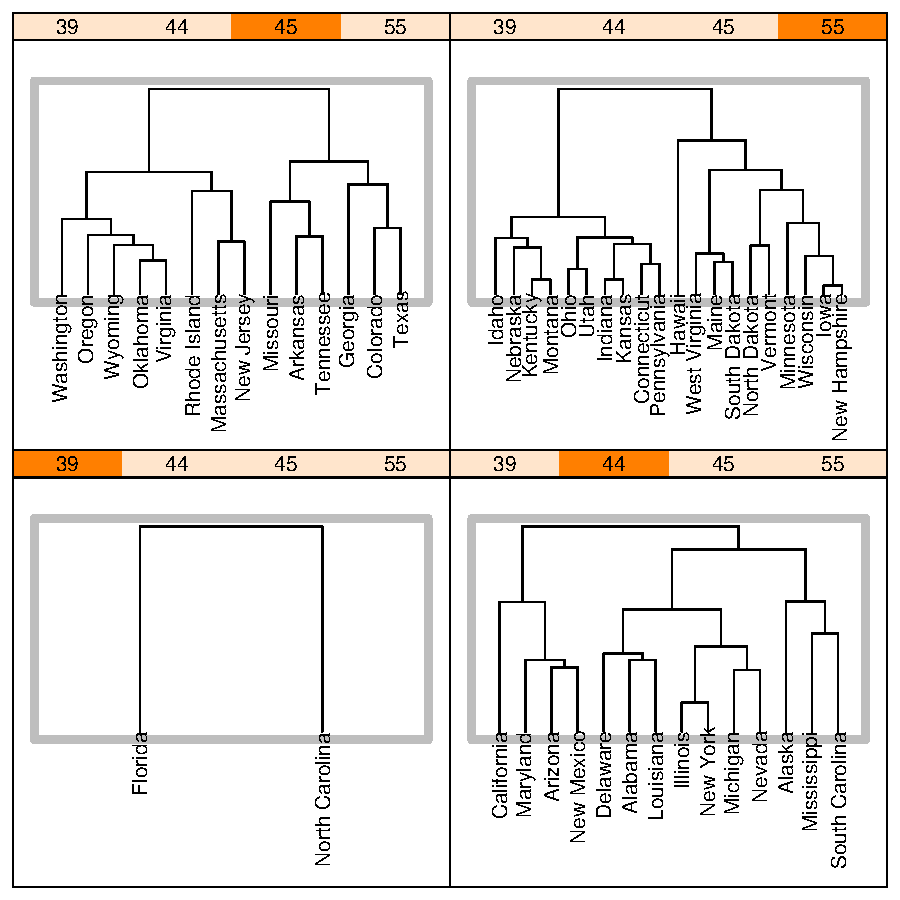
\includegraphics{gridBase-014}

The \verb|gridPLT()| function is useful for embedding just the
plot region of a base graphics function (i.e., without labels and
axes;  another example of this usage 
is given in the next section).  If labelling
and axes are to be included it will make more sense to use
\verb|gridFIG()|.  The \verb|gridOMI()| function has pretty much
the same effect as \verb|gridFIG()| except that it allows for the
possibility of embedding multiple base plots at once.  In the
following code, a \lattice{} plot is placed alongside 
base diagnostic plots arranged in a 2-by-2 array.

We use the data from page 93 of
``An Introduction to Generalized Linear Models'' (Annette Dobson, 1990).

\begin{Schunk}
\begin{Sinput}
> counts <- c(18, 17, 15, 20, 10, 20, 25, 13, 12)
> outcome <- gl(3, 1, 9)
> treatment <- gl(3, 3)
\end{Sinput}
\end{Schunk}
We create two regions using \grid{} viewports;  the left region
is for the \lattice{} plot and the right region is for the diagnostic
plots.  There is a middle column of 1cm to provide a gap between
the two regions.

% Save and restore settings so that vignette building will work(?)
\begin{Schunk}
\begin{Sinput}
> pushViewport(viewport(layout = grid.layout(1, 3, widths = unit(rep(1, 
+     3), c("null", "cm", "null")))))
\end{Sinput}
\end{Schunk}
We draw a \lattice{} plot in the left region.

\begin{Schunk}
\begin{Sinput}
> pushViewport(viewport(layout.pos.col = 1))
> library(lattice)
> bwplot <- bwplot(counts ~ outcome | treatment)
> print(bwplot, newpage = FALSE)
> popViewport()
\end{Sinput}
\end{Schunk}
We draw the diagnostic plots in the right region.  Here
we use \verb|gridOMI()| to set the base inner region and
\verb|par(mfrow)| and 
\verb|par(mfg)| to insert multiple plots\footnote{We use
{\tt par(mfrow)} to specify the 2-by-2 array
and {\tt par(mfg)} to start at position $(1,1)$ in the 
array.}.

\begin{Schunk}
\begin{Sinput}
> pushViewport(viewport(layout.pos.col = 3))
> glm.D93 <- glm(counts ~ outcome + treatment, family = poisson())
> par(omi = gridOMI(), mfrow = c(2, 2), new = TRUE)
> par(cex = 0.5, mar = c(5, 4, 1, 2))
> par(mfg = c(1, 1))
> plot(glm.D93, caption = "", ask = FALSE)
> popViewport(2)
\end{Sinput}
\end{Schunk}
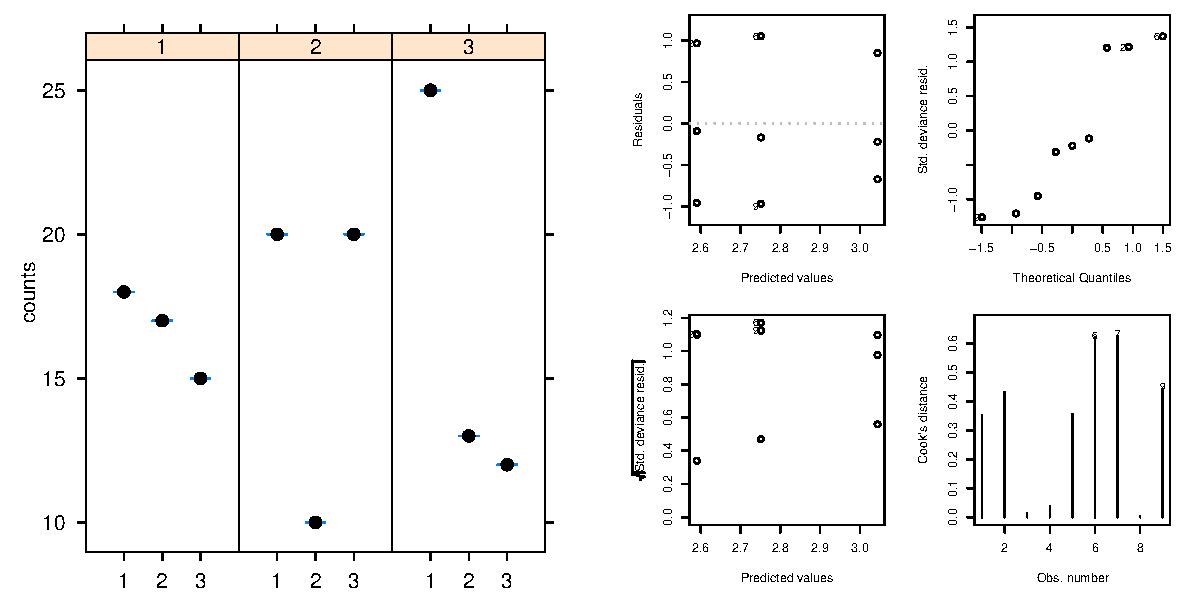
\includegraphics[width=5in]{gridBase-multiplot}

% Save and restore settings so that vignette building will work(?)
Notice that because there is only ever one current \grid{} viewport, it only 
makes sense to use one of \verb|gridOMI()|, \verb|gridFIG()|, or
\verb|gridPLT()|.  In other words, it only makes sense to 
align either the inner region, or the figure region, or the plot
region with the current \grid{} viewport.

\section*{A more complex example}

We will now look at a reasonably complex example involving
embedding base graphics within grid viewports which are themselves
embedded within a base plot.  This example is motivated by
 the following problem\footnote{This description is from an email to 
R-help from Adam Langley, 18 July 2003}:

\begin{quote}
I am looking at a way of plotting a series of pie charts at specified
locations on an existing plot. The size of the pie chart would be proportion
to the magnitude of the total value of each vector (x) and the values in x
are displayed as the areas of pie slices.
\end{quote}

First of all, we construct some fake data, consisting of four
$(x, y)$ values, and four $(z_1, z_2)$ values :

\begin{Schunk}
\begin{Sinput}
> x <- c(0.88, 1, 0.67, 0.34)
> y <- c(0.87, 0.43, 0.04, 0.94)
> z <- matrix(runif(4 * 2), ncol = 2)
\end{Sinput}
\end{Schunk}
Before we start any plotting, we save the current \verb|par()| 
settings so that at the end 
we can ``undo'' some of the complicated settings
that we need to apply.

\begin{Schunk}
\begin{Sinput}
> oldpar <- par(no.readonly = TRUE)
\end{Sinput}
\end{Schunk}
Now we do a standard base plot of the $(x, y)$ values, but do not
plot  anything at these locations (we're just setting up the
user coordinate system).

\begin{Schunk}
\begin{Sinput}
> plot(x, y, xlim = c(-0.2, 1.2), ylim = c(-0.2, 1.2), type = "n")
\end{Sinput}
\end{Schunk}
Now we make use of \verb|baseViewports|.
This will create a list of grid viewports that correspond to the 
inner, figure, and plot regions set up by the base plot.
By pushing these viewports, we establish a grid viewport that aligns
exactly with the plot region created by the base plot, including a
(grid) ``native'' coordinate system that matches the
(base) user coordinate system\footnote{
The {\tt grid.segments} call is just drawing some 
dashed lines to show that the pie charts we end up with 
are centred correctly at the appropriate $(x, y)$ locations.}.

\begin{Schunk}
\begin{Sinput}
> vps <- baseViewports()
> par(new = TRUE)
> pushViewport(vps$inner, vps$figure, vps$plot)
> grid.segments(x0 = unit(c(rep(0, 4), x), rep(c("npc", "native"), 
+     each = 4)), x1 = unit(c(x, x), rep("native", 8)), y0 = unit(c(y, 
+     rep(0, 4)), rep(c("native", "npc"), each = 4)), y1 = unit(c(y, 
+     y), rep("native", 8)), gp = gpar(lty = "dashed", col = "grey"))
\end{Sinput}
\end{Schunk}
Before we draw the pie charts, we need to perform a couple of
calculations to determine their size.  In this case, we specify that
the largest pie will be 1\verb|"| in diameter and the others will be 
a proportion of that size based on $\sum_i{z_{.i}} /
{\mathrm{max}}\left( \sum_i{z_{.i}} \right)$

\begin{Schunk}
\begin{Sinput}
> maxpiesize <- unit(1, "inches")
> totals <- apply(z, 1, sum)
> sizemult <- totals/max(totals)
\end{Sinput}
\end{Schunk}
We now enter a loop to draw a pie at each $(x, y)$ location
representing the corresponding $(z_1, z_2)$ values.  The first
step is to create a grid viewport at the $(x, y)$ location,
then we use \verb|gridPLT()|
to set the base plot region to correspond to the grid viewport.
With that done, we can use the base \verb|pie| function to draw a pie
chart within the grid viewport\footnote{We draw a {\tt grid.rect} 
with a dashed border just to show the extent of each grid viewport.
It is crucial that we again call {\tt par(new=TRUE)} so that
we do not move on to a new page.}.  

\begin{Schunk}
\begin{Sinput}
> for (i in 1:4) {
+     pushViewport(viewport(x = unit(x[i], "native"), y = unit(y[i], 
+         "native"), width = sizemult[i] * maxpiesize, height = sizemult[i] * 
+         maxpiesize))
+     grid.rect(gp = gpar(col = "grey", fill = "white", lty = "dashed"))
+     par(plt = gridPLT(), new = TRUE)
+     pie(z[i, ], radius = 1, labels = rep("", 2))
+     popViewport()
+ }
\end{Sinput}
\end{Schunk}
Finally, we clean up after ourselves by popping the grid viewports
and restoring the initial \verb|par| settings.

\begin{Schunk}
\begin{Sinput}
> popViewport(3)
> par(oldpar)
\end{Sinput}
\end{Schunk}
The final plot is shown below.

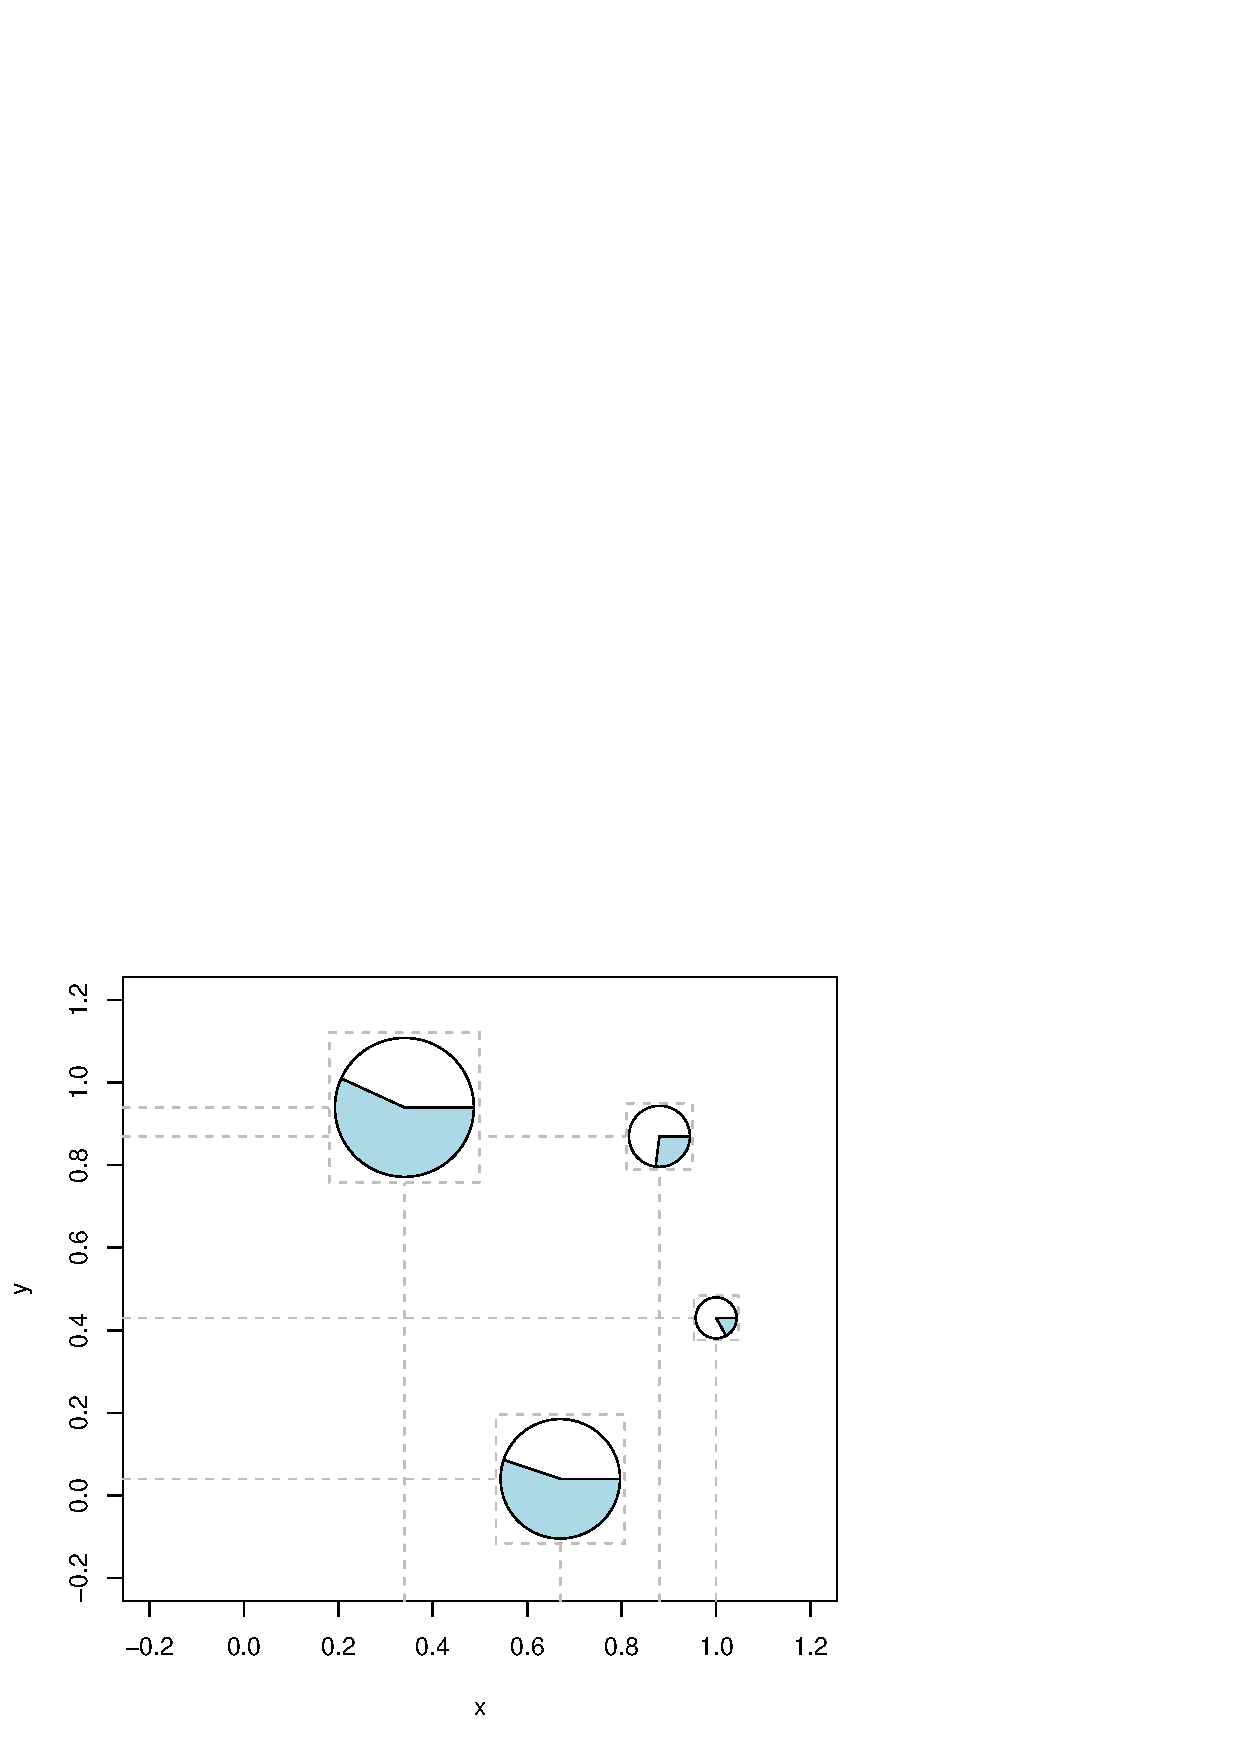
\includegraphics{gridBase-complex}
\section*{Problems and limitations}

The functions provided by the \gridBase{} package allow the user
to mix output from two quite different graphics systems and there 
are limits to how much the systems can be combined.  It is important
that users are aware that they are mixing two not wholly compatible
systems (which is why these functions are provided in a separate 
package) and it is of course important to know what the limitations
are: 

\begin{itemize}
\item 
The \gridBase{} functions attempt to
match \grid{} graphics settings with base graphics settings (and vice versa). 
 This 
is only possible under certain conditions.  For a start, it is only 
possible if the device size does not change.  If these functions are
used to draw into a window,  then the window is resized, the base and 
\grid{} settings will almost certainly no longer match and the graph
will become a complete mess.  This also applies to copying output between
devices of different sizes.

\item
It is not possible to embed base graphics output within a 
\grid{} viewport that is rotated.

\item
There are certain base graphics functions 
which modify settings
like \verb|par(omi)| and \verb|par(fig)| themselves (e.g., \verb|coplot()|).
  Output from
these functions may not embed properly
within \grid{} viewports.

\item
\grid{} output cannot be
saved and restored so any attempts to save a mixture of \grid{} and
base output are likely
to end in disappointment.

\end{itemize}

\section*{Summary}

The functions in the \gridBase{} package provide a simple mechanism
for combining base graphics output with \grid{} graphics output
for static, fixed-size plots.  This is not a full integration
of the two graphics systems, but it does provide a useful bridge
between the existing large body of base graphics functions and the
powerful new features of \grid{}.


\subsubsection*{Availability}

The \grid{} package is now part of the base distribution of \R{}
(from \R{} version 1.8.0).  \\
Additional information on \grid{}
is available from:\\
 {\tt http://www.stat.auckland.ac.nz/~paul/grid/grid.html}. \\
The \gridBase{} package
is available from \verb|CRAN| (e.g., {\tt http://cran.us.r-project.org}).

\bibliographystyle{plain}
\bibliography{gridBase}

\end{document}

We use the Plant Weight Data from 
``An Introduction to Generalized Linear Models'' (Annette Dobson, 1990).

\begin{Schunk}
\begin{Sinput}
> ctl <- c(4.17, 5.58, 5.18, 6.11, 4.5, 4.61, 5.17, 4.53, 5.33, 
+     5.14)
> trt <- c(4.81, 4.17, 4.41, 3.59, 5.87, 3.83, 6.03, 4.89, 4.32, 
+     4.69)
> group <- gl(2, 10, 20, labels = c("Ctl", "Trt"))
> weight <- c(ctl, trt)
\end{Sinput}
\end{Schunk}
We create two regions using \grid{} viewports;  the left region
is for the \lattice{} plot and the right region is for the diagnostic
plots.  There is a middle column of 1cm to provide a gap between
the two regions.

% Save and restore settings so that vignette building will work(?)
\begin{Schunk}
\begin{Sinput}
> pushViewport(viewport(layout = grid.layout(1, 3, widths = unit(rep(1, 
+     3), c("null", "cm", "null")))))
\end{Sinput}
\end{Schunk}
We draw a \lattice{} plot in the left region.

\begin{Schunk}
\begin{Sinput}
> pushViewport(viewport(layout.pos.col = 1))
> library(lattice)
> bwplot <- bwplot(weight ~ group)
> print(bwplot, newpage = FALSE)
> popViewport()
\end{Sinput}
\end{Schunk}
We draw the diagnostic plots in the right region.  Here
we use \verb|gridOMI()| to set the base inner region and
\verb|par(mfrow)| and 
\verb|par(mfg)| to insert multiple plots\footnote{We use
{\tt par(mfrow)} to specify the 2-by-2 array
and {\tt par(mfg)} to start at position $(1,1)$ in the 
array.}.

\begin{Schunk}
\begin{Sinput}
> pushViewport(viewport(layout.pos.col = 3))
> lm.D9 <- lm(weight ~ group)
> par(omi = gridOMI(), mfrow = c(2, 2), new = TRUE)
> par(cex = 0.5)
> par(mfg = c(1, 1))
> plot(lm.D9, caption = "", ask = FALSE)
> popViewport(2)
\end{Sinput}
\end{Schunk}
